\begin{figure}[h!]
\centering

% --- Grouped bar chart: three comparable metrics on [0, 100] scale ---
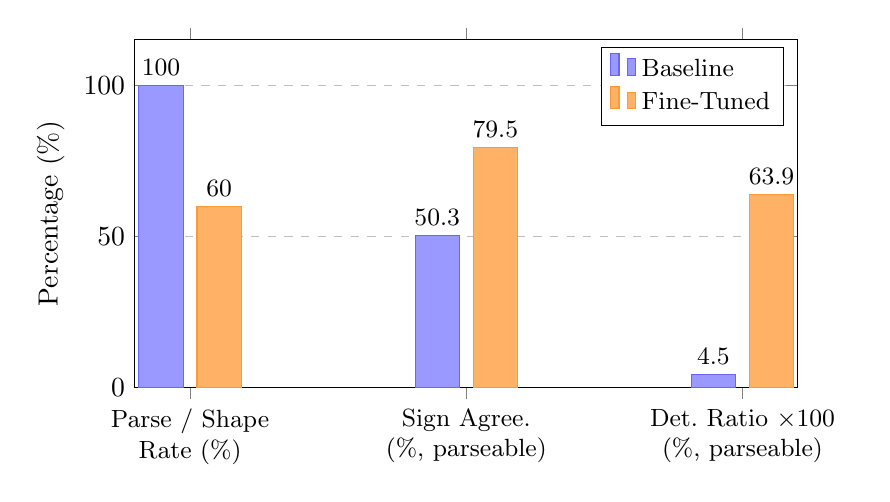
\begin{tikzpicture}
\begin{axis}[
    width=10cm,
    height=6cm,
    ylabel={Percentage (\%)},
    ybar=5pt,
    bar width=16pt,
    ymin=0,
    ymax=115,
    xtick=data,
    xticklabels={
        {Parse / Shape\\Rate (\%)},
        {Sign Agree.\\(\%, parseable)},
        {Det.\ Ratio $\times 100$\\(\%, parseable)}
    },
    x tick label style={font=\small, align=center, text width=2.8cm},
    legend style={at={(0.98,0.98)}, anchor=north east, font=\small},
    legend cell align={left},
    ymajorgrids=true,
    grid style=dashed,
    nodes near coords,
    nodes near coords align={vertical},
    every node near coord/.append style={font=\small},
]
\addplot[fill=blue!40, draw=blue!60] coordinates {
    (1, 100.0)
    (2, 50.3)
    (3, 4.5)
};
\addplot[fill=orange!60, draw=orange!80] coordinates {
    (1, 60.0)
    (2, 79.5)
    (3, 63.9)
};
\legend{Baseline, Fine-Tuned}
\end{axis}
\end{tikzpicture}

\vspace{0.8cm}

% --- Failure mode bar chart: fine-tuned model ---
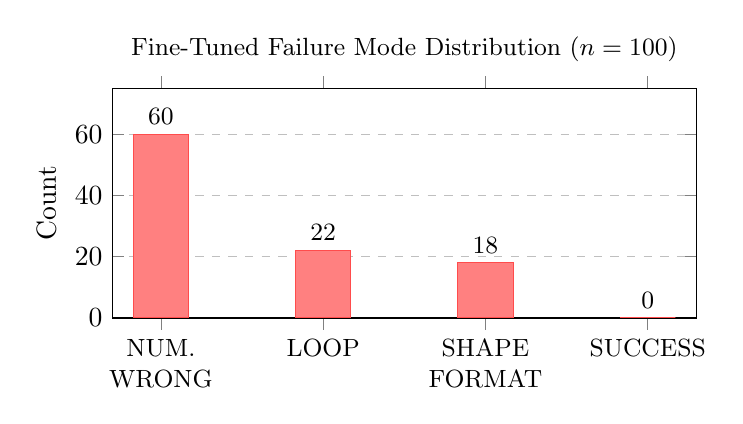
\begin{tikzpicture}
\begin{axis}[
    width=9cm,
    height=4.5cm,
    title={Fine-Tuned Failure Mode Distribution ($n = 100$)},
    title style={font=\small},
    ylabel={Count},
    ybar,
    bar width=20pt,
    ymin=0,
    ymax=75,
    xtick=data,
    xticklabels={
        {NUM.\\WRONG},
        {LOOP},
        {SHAPE\\FORMAT},
        {SUCCESS}
    },
    x tick label style={font=\small, align=center},
    ymajorgrids=true,
    grid style=dashed,
    nodes near coords,
    nodes near coords align={vertical},
    every node near coord/.append style={font=\small},
]
\addplot[fill=red!50, draw=red!70] coordinates {
    (1, 60)
    (2, 22)
    (3, 18)
    (4, 0)
};
\end{axis}
\end{tikzpicture}

\caption{
\textbf{Top}: Three normalized metrics (all higher = better) comparing baseline and fine-tuned model. Parse/shape rate measures generation reliability; sign agreement and determinant ratio ($\times 100$ for scale) measure inverse-like coarse structure among parseable outputs. Fine-tuning improves both structural metrics---sign agreement rises from 50.3\% to 79.5\%, determinant ratio from 4.5\% to 63.9\%---but reduces parse reliability by 40 percentage points. Additional diagnostics (residuals, relative Frobenius error, spectral error, copy distances) are in Table~\ref{tab:results}.
\textbf{Bottom}: Failure mode distribution for the fine-tuned model ($n = 100$ test examples). 60 outputs are parseable but numerically wrong; 22 loop until the token budget is exhausted; 18 produce malformed shapes; 0 achieve a successful inversion.}
\label{fig:results}
\end{figure}
